\documentclass[11pt]{article}
\usepackage[margin=2.6cm]{geometry}
\usepackage{mathpazo}
\usepackage{amsmath}
\usepackage{microtype}
\usepackage{booktabs}
\usepackage{pgfplots}
\pgfplotsset{compat=1.16}
\usepackage[font=small,labelfont=bf]{caption}
\usepackage{titlesec}
\titleformat{\section}{\large\bfseries}{\thesection}{0.8em}{}
\titleformat{\subsection}{\normalsize\bfseries\itshape}{\thesubsection}{0.8em}{}
\setlength{\parskip}{0.55em}
\setlength{\parindent}{0pt}
\begin{document}

\begin{center}
{\LARGE\bfseries A Comfort Reward With a Price on Time}\\[0.5em]
{\large Reward design of the CALM speed recommender}
\end{center}
\vspace{0.6em}

\section{Purpose}

The policy recommends how far to slow down before a speed bump. A bump is crossed more comfortably at low speed, so a reward that measures comfort alone is maximised by crawling over every road. A useful reward must therefore weigh comfort against the time the trip takes, and it must do so in a way that is comparable between a mild road and a severe one. This document describes how the reward achieves both.

\section{Decision and speed command}

The policy makes one decision per bump. When the car is $25$\,m before a bump, it chooses a depth $d \in \{0,\ 0.65,\ 0.85\}$. The environment then ramps the speed towards
\begin{equation}
v_{\text{target}} = v_0 - (v_0 - v_{\text{low}})\; d \; w(s),
\end{equation}
where $v_0$ is the scenario speed, $v_{\text{low}} = 5$\,km/h is the speed floor and $w(s)\in[0,1]$ is a smooth window that rises $25$ to $8$\,m before the bump and falls back $4$\,m after the rear axle has left it. The timing of the slowdown is therefore fixed by the environment, and the policy only learns how deep to go. The reward below is collected every simulation step of $\Delta t = 0.02$\,s and once at the end of the road; the decision step receives the sum of the steps it covers.

\section{Comfort cost}

Passenger discomfort is measured by the vertical acceleration of the car body $a_{B,k}$ after the ISO 2631-1 Wk frequency weighting, which emphasises the frequencies the human body is most sensitive to. At step $k$,
\begin{equation}
J^{B}_k = -\Big(\frac{a_{B,k}}{g}\Big)^{2}, \qquad g = 9.81\ \mathrm{m/s^2}.
\end{equation}
The comfort cost of a drive is $C = -\sum_k Q_B J^{B}_k$, with weight $Q_B = 50$. Three small terms keep the speed profile smooth and are not part of the comfort measure itself: the longitudinal acceleration $J^{a}_k = -(a_k/g)^2$, its change per step $J^{j}_k = -((a_k - a_{k-1})/g)^2$ and $J^{s}_k = -((a_k - a_{k-1})/a_{\max})^2$ with $a_{\max} = 5$\,m/s$^2$, weighted by $Q_a = 0.2$, $w_j = 0.4$ and $w_s = 0.2$. The base step reward is
\begin{equation}
r^{0}_k = Q_B J^{B}_k + Q_a J^{a}_k + w_j J^{j}_k + w_s J^{s}_k .
\end{equation}

\section{The reference drive and the frontier}

The comfort cost of a road depends mostly on the road. A severe bump produces a large $C$ at any speed, so raw costs cannot be compared between roads and a policy would be rewarded for easy roads. Each road therefore gets its own yardstick: the same road driven at constant speed.

Before the episode, the road is driven at eight constant speeds $v_i$ between $v_{\text{low}}$ and $v_0$. Each drive takes a time $T_i$ and has a comfort cost $C_i$. Slower drives take longer and are more comfortable, so the points $(T_i, C_i)$ form a falling curve, the \emph{frontier} $C_c(T)$ (Figure~\ref{fig:frontier}). It answers the question: how comfortable can a constant speed be if it may take time $T$? The fastest drive, at $v_0$, is the \emph{reference}, with cost $C_{\text{ref}}$ and time $T_{\text{ref}}$. Costs are never allowed below $C_{\min} = 1$.

\begin{figure}[t]
\centering
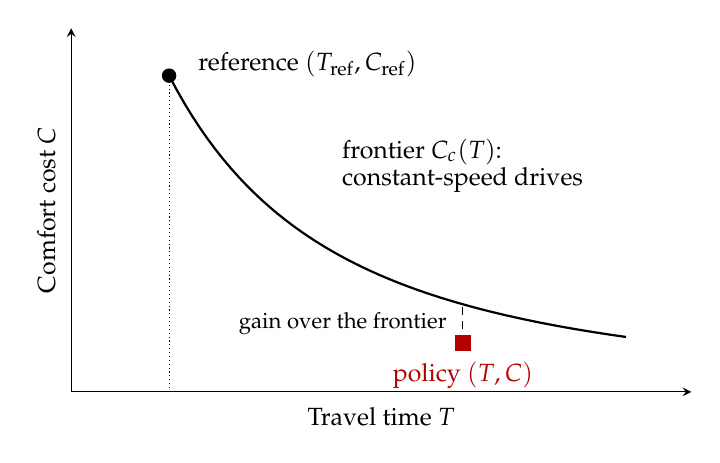
\begin{tikzpicture}
\begin{axis}[
  width=0.78\linewidth, height=6.2cm,
  xlabel={Travel time $T$}, ylabel={Comfort cost $C$},
  xmin=0.7, xmax=2.6, ymin=0, ymax=4.6,
  xtick=\empty, ytick=\empty, axis lines=left, clip=false,
  every axis label/.append style={font=\small}]
\addplot[thick, domain=1:2.4, samples=60] {1/(x*x)*4};
\node[font=\small, anchor=south west] at (axis cs:1.5,2.75) {frontier $C_c(T)$:};
\node[font=\small, anchor=south west] at (axis cs:1.5,2.4) {constant-speed drives};
\addplot[only marks, mark=*, mark size=2.4pt] coordinates {(1,4)};
\node[font=\small, anchor=west] at (axis cs:1.06,4.15) {reference $(T_{\mathrm{ref}},C_{\mathrm{ref}})$};
\addplot[only marks, mark=square*, mark size=2.6pt, red!70!black] coordinates {(1.9,0.62)};
\node[font=\small, anchor=north, red!70!black] at (axis cs:1.9,0.5) {policy $(T,C)$};
\draw[densely dashed] (axis cs:1.9,0.62) -- (axis cs:1.9,1.108);
\node[font=\footnotesize, anchor=east, fill=white, inner sep=1pt] at (axis cs:1.86,0.86) {gain over the frontier};
\draw[densely dotted] (axis cs:1,0) -- (axis cs:1,4);
\end{axis}
\end{tikzpicture}
\caption{Illustration of the frontier. The policy is judged against a constant-speed drive that takes the same time $T$, not against the fast reference.}\label{fig:frontier}
\end{figure}

\section{Scaling by the reference}

Dividing by the reference cost makes the reward independent of how severe the road is. Each step is scaled so that a constant drive at $v_0$ collects about $-K$ on every road, with $K = 100$:
\begin{equation}
r^{1}_k = \frac{K}{C_{\text{ref}}}\,Q_B J^{B}_k + Q_a J^{a}_k + w_j J^{j}_k + w_s J^{s}_k .
\end{equation}
The longitudinal terms are left unscaled. The result is a dense signal at every step that has the same meaning on every road.

\section{Time price}

Scaling alone would still reward crawling, because slower driving always lowers $C$. Time is therefore priced through the lag behind the reference drive. After distance $s_k$ in time $t_k$,
\begin{equation}
\ell_k = \max\!\Big(t_k - \frac{s_k}{v_0},\ 0\Big).
\end{equation}
The lag is zero while the car is at least as fast as the reference drive and grows by one second for every second the car spends standing still. The price per step is quadratic in the lag and scaled by the reference time,
\begin{equation}
p_k = \kappa\, K \Big(\frac{\ell_k}{T_{\text{ref}}}\Big)^{2}\frac{\Delta t}{T_{\text{ref}}}, \qquad \kappa = 0.9, \qquad r_k = r^{1}_k - p_k .
\end{equation}
Two properties are intended. A small delay is almost free, because the price grows with the square of the lag, so the policy may slow down for severe bumps. A long delay is expensive, so it cannot crawl. And because the lag is measured in units of $T_{\text{ref}}$, the same slowdown costs the same fraction of the reward on a short road and on a long one. The factor $\kappa$ sets the exchange rate between comfort and time. It was chosen with a scan over several values; the result is a comfort-versus-time trade, not a free gain.

\section{End of the road}

At the end of the drive the car has taken a time $T$ and incurred a total comfort cost $C$. The summed step rewards contain the comfort part $-K\,C/C_{\text{ref}}$, which compares against the \emph{fast} reference. A terminal term replaces it by the comparison with the constant drive of the \emph{same} time:
\begin{equation}
F = -K\,C\left(\frac{1}{C_c(T)} - \frac{1}{C_{\text{ref}}}\right),
\qquad
-K\frac{C}{C_{\text{ref}}} + F = -K\,\frac{C}{C_c(T)} .
\end{equation}
The comfort reward over the episode is therefore $-K\,C/C_c(T)$. It equals $-K$ when the policy is exactly as comfortable as a constant drive of the same duration, and it is better than $-K$ when the policy beats it. This is the equal-time comparison of the evaluation (Figure~\ref{fig:frontier}), built into the training signal, and it is why driving slower is not rewarded on its own. A road completed earns a bonus $R_{+} = 100$; an episode that ends in failure receives $R_{-} = -250$ instead. The episode return is the sum of the step rewards and the terminal reward,
\begin{equation}
G = \sum_{k=1}^{N} r_k + \big(D + F\big), \qquad D \in \{R_{+},\, R_{-}\}.
\end{equation}

\section{Limits}

The reference and the frontier are computed with the same simulated vehicle and the road known exactly, so the reward cannot be evaluated on a real car; it is a training device. Because the slowdown timing is fixed by the environment, the reward shapes the depth of the slowdown only. The exchange rate $\kappa$ was selected with a scan that touched some of the held-out roads.

\end{document}
